%Automation of Biological Research 
%Project Image Classification
%due Dec/11/2016
%Email responses to: ABR-instructors@googlegroups.com
%Landmark Clustering
\documentclass{article}
\usepackage{amsmath}
\usepackage{amssymb}
\usepackage{amsfonts}
\usepackage{graphicx}
\usepackage{listings}
\usepackage{qtree}
\usepackage{pgf}
\usepackage{tikz}
\usetikzlibrary{arrows,automata}
\usepackage[latin1]{inputenc}
\usepackage{verbatim}
\usepackage{fullpage}
\usepackage{algpseudocode}
\usepackage{algorithm}
\usepackage{hyperref}
\usepackage{cleveref}
\usepackage{courier}

%\usetikzlibrary{arrows}

\usepackage{indentfirst}
\newcommand{\E}{\mathrm{E}}
\newcommand{\Var}{\mathrm{Var}}
\newcommand{\Cov}{\mathrm{Cov}}
\newcommand{\T}{\mathrm{T}}
\newcommand{\F}{\mathrm{F}}
\newcommand\independent{\protect\mathpalette{\protect\independenT}{\perp}}
\def\independenT#1#2{\mathrel{\rlap{$#1#2$}\mkern2mu{#1#2}}}
%\setlength{\parindent}{1cm} % Default is 15pt.



\begin{document}

\title{Automation of Biological Research Course Project-2016fall}
\author{Yanyu Liang \\ yanyul@andrew.cmu.edu \and Priyanka Raja \\ priyankj@andrew.cmu.edu}

\maketitle

% \section{Memo}

% \subsection{PCA analysis}
%   In passive learning (randomly select 2500 samples from the pool), sparse logistic regression can succcessful filter out unrelated features. Evidence is from PCA analysis shown in \Cref{fig:pca1}  and \Cref{fig:pca2}. 
%   \begin{figure}[!ht]
%     \begin{minipage}{.45\textwidth}
%       \centering
%       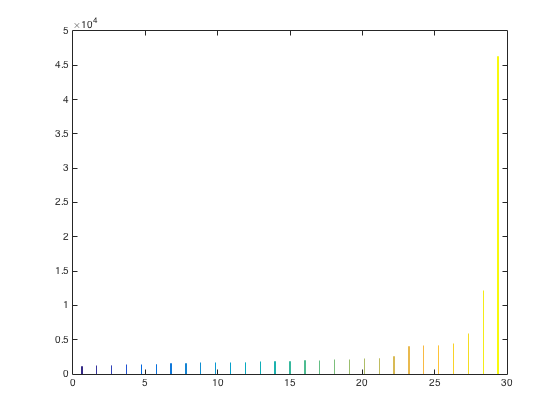
\includegraphics[width=1\linewidth]{pca1}
%       \caption{PCA on nonzero features}
%       \label{fig:pca1}
%     \end{minipage}
%     \hfill
%     \begin{minipage}{.45\textwidth}
%       \centering
%       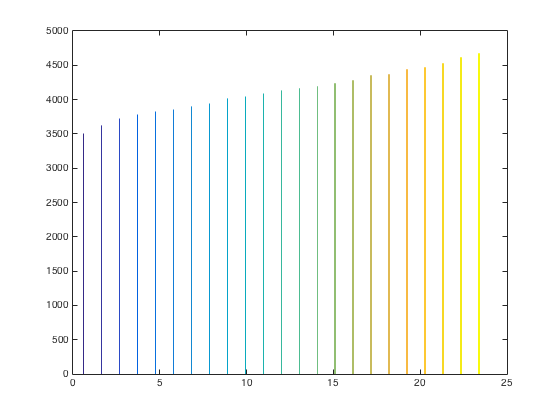
\includegraphics[width=1\linewidth]{pca2}
%       \caption{PCA on zero features}
%       \label{fig:pca2}
%     \end{minipage}
%   \end{figure}
%   It seems that normalization itself helps a lot here \Cref{fig:pca_results_moderate_50}.
%   With PCA as preprocessing (explaining 50\% or 90 \%), the results are worse than before.
%   \begin{figure}[!ht]
%     \centering
%     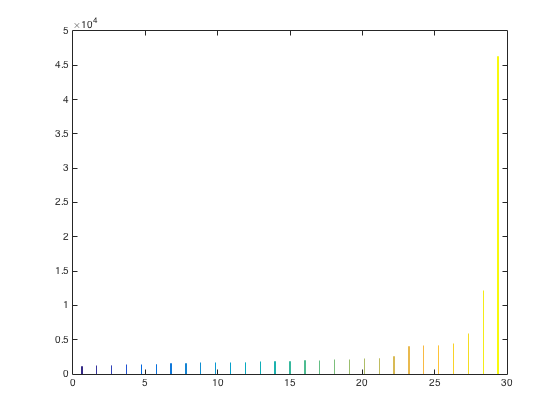
\includegraphics[width=1\linewidth]{pca1}
%     \caption{Normalization as preprocessing}
%     \label{fig:pca_results_moderate_50}
%   \end{figure}

\section{Methods Overview}


In this project, the data is $(x, y)$ and our task is to build a classifier to infer the label $y$ given $x$ under pool based active learning setting. We used uncertainty sampling as our active learning algorithm. To implement this approach, one requirement for the base learner is that it should assign probability to each label, namely $\Pr(Y = c_i|X = x, \text{model}), \forall i = 1, ..., k$.


\subsection{Active learning strategy - Uncertainty sampling}


Specifically, the uncertainty sampling approach we implemented is Best-versus-Second Best (BvSB) \cite{joshi2009multi}. At each iteration, for each unlabeled sample in the pool, we first compute $\vec{p} = (p_1, ..., p_k)^T$, where $p_i = \Pr(Y = c_i|X = x, \text{model})$ using our current classifier. And then the BvSB score is computed as follow:
\begin{align*}
  \text{BvSB} &= p_{(1)} - p_{(2)} \\
  \text{,where } p_{(1)} &= p_j = \arg\max_{j} p_j \\
  p_{(2)} &= p_l = \arg\max_{l \neq j} p_l
\end{align*}
Namely, BvSB is the difference between the probabilities of the most probable class and the second most probable class. Although entropy measure (EP) is widely used in uncertainty sampling, in multi-class problem, EP might not be suitable because in the case where $vec{p}$ has a heavy tail (even if the most probable class clearly stands out). In this sense, BvSB is more robust and we implemented BvSB as the uncertainty measure. And the active learner always queries the data point which has lowest BvSB score.

\subsection{Base learners}

The uncertainty sampling approach requires the base learner has probabilistic interpretation of label assignment. To achieve this, logistic regression is a natural choice. Other than this, with the use of softmax function at the output layer, neural network can be seen as a machinery to fit the function $\Pr(Y = y|X = x)$ which is also suitable in this set up. Hence, in these two classifiers, the learning objective is the negative log likelihood function. 

Alternatively, we also applied SVM as base learner. SVM is widely used in binary classification and it is often known as a maximum margin classifier without probabilistic explanation. However, in one-vs-one approach for multi-class SVM implementation, the distance to each decision hyperplane can be transferred into a probabilistic interpretation \cite{wu2004probability}. So, we also used SVM as one of our base learners and we directly applied \texttt{libsvm} package \cite{CC01a}.

Furthermore, to overcome overfitting, we regularized our logistic regression classifier and neural network classifier (one hidden layer with the number of nodes equals to 3 times the number of features) using both $l_1$ and $l_2$ penalties. We implemented the optimization algorithms of these two from sketch and in every iteration, we treated the previous model as a warm start and this made tremendously saved the computing power.

\subsection{Implementation details}


In the implementation, we used warm start, namely to randomly select 10 points from the pool to build the initial classifier. The reason why we use warm start instead of cold start is that SVM is built from a collection of binary classifiers and most of the sub-classifiers will be empty in cold start, which is potentially a technical issue. Furthermore, at the very beginning, the classifier is not very trustable for the sake of lack of data. 


For the base learners, we set up kernels and hyperparameters as follow. The kernel of SVM was set as RBF kernel with default parameters. The hyperparameters of logistic regression is 10 for $l_2$ regularizer and 50 for group lasso regularizer. And the hyperparameters of neural network, namely group lasso, $l_2$ regularizer of $W_1$ and $l_2$ regularizer of $W_2$ are all set to 1, where $W_i$ is the linear connection between $i$th layer and $(i+1)$th layer. The design of group lasso penalty is as follow:
\begin{align*}
  \text{group lasso on } W = \sum_i \|W_i\|_2
\end{align*}
, where $W_i$ is the $i$th row of $W$ which are the coefficients of $i$th feature. In another word, this term penalizes all of the coefficients of $i$th feature as a group and this can, on one hand, avoid overfitting and on the other hand, perform feature selection. Furthermore, the proximal gradient descent with backtracking was used for the training of both logistic regression and the neural network.

\section{Results}

In this section, we show the results of our three base learners along with uncertainty sampling one by one. Here, logistic regression is referred as sparseLogit and neural network is referred as sparseNN.

\subsection{Base learner - SVM}

The results of uncertainty sampling with SVM as base learner is shown in \Cref{fig:svm}. The y-axis is the rate of test error along learning and the x-axis is the number of queries (same for all the figures below if not specified).
  \begin{figure}[!ht]
    \begin{minipage}{.31\textwidth}
      \centering
      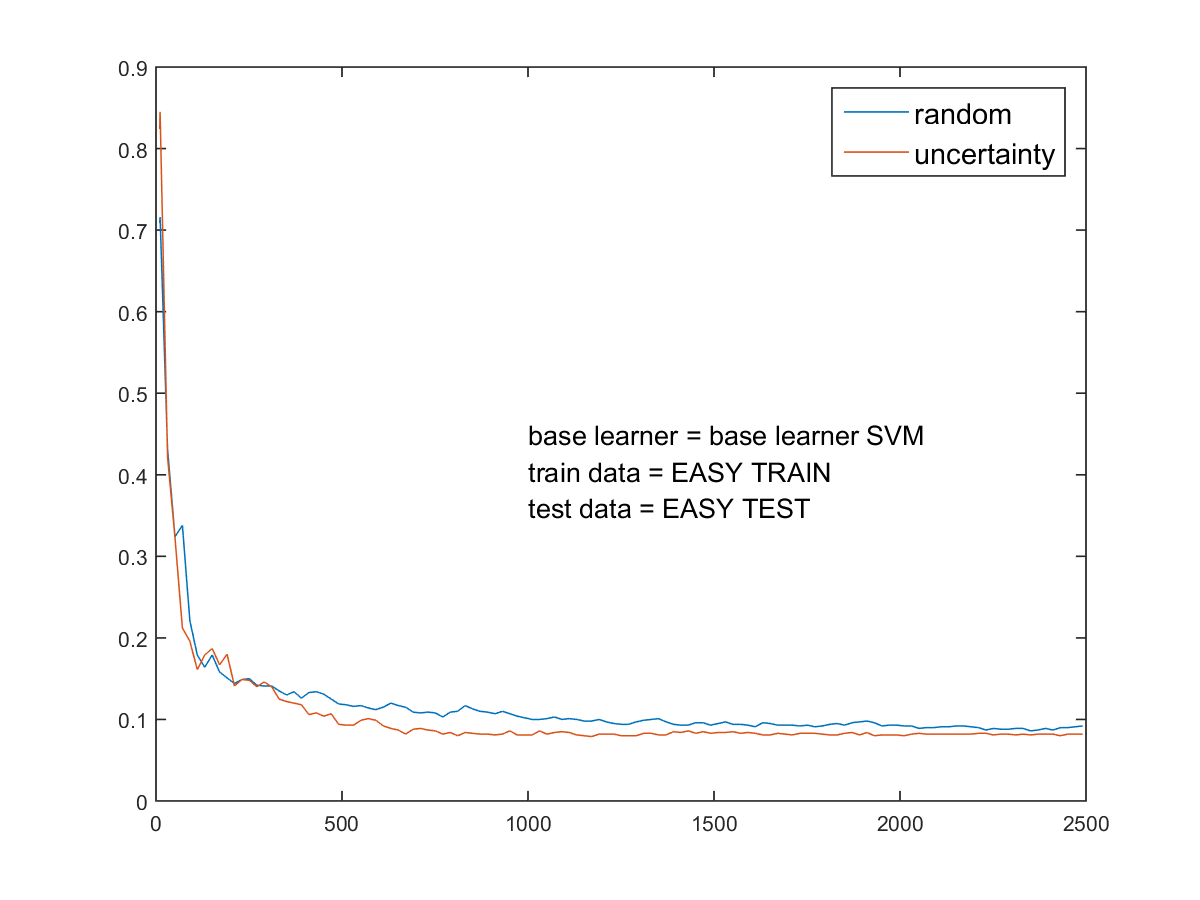
\includegraphics[width=1\linewidth]{../svm_simple}
    \end{minipage}
    \hfill
    \begin{minipage}{.31\textwidth}
      \centering
      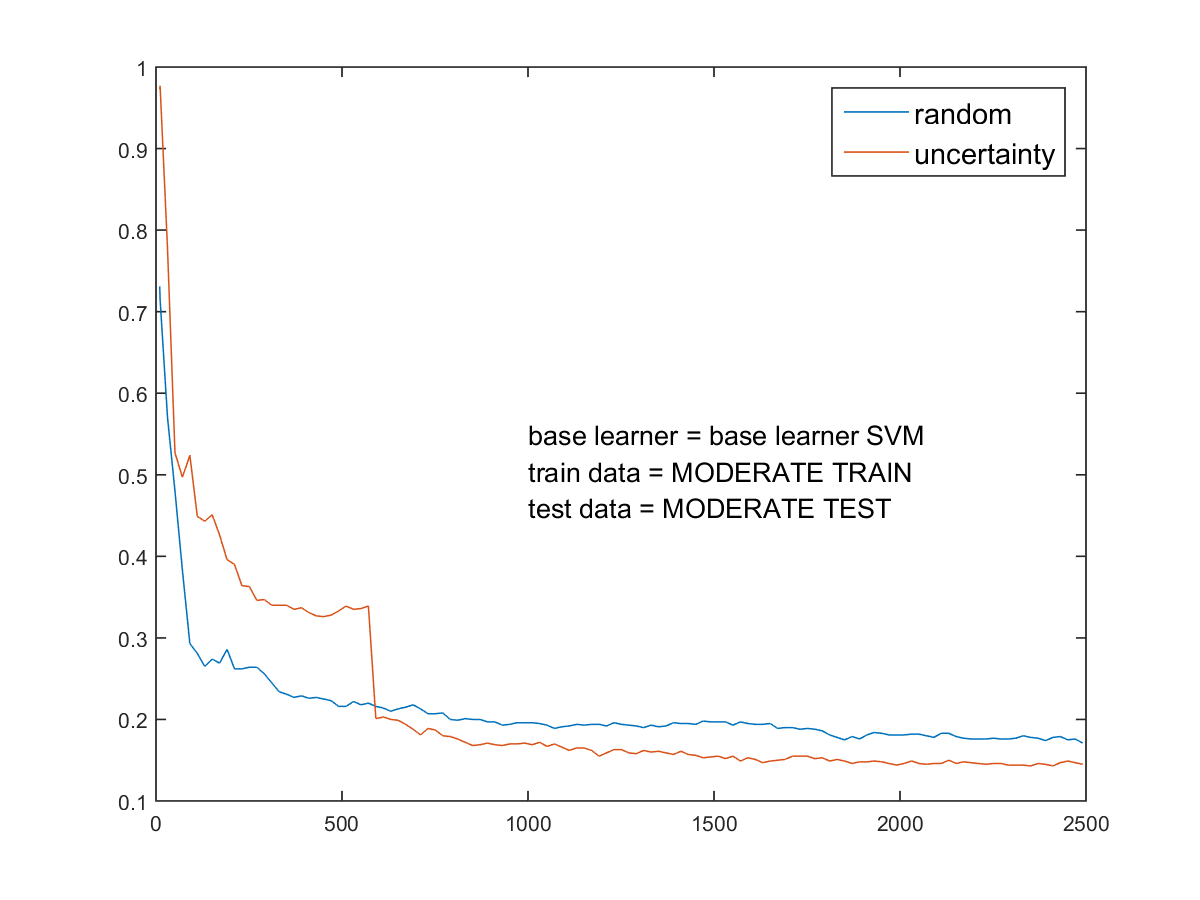
\includegraphics[width=1\linewidth]{../svm_moderate}
    \end{minipage}
    \hfill
    \centering
    \begin{minipage}{.31\textwidth}
      \centering
      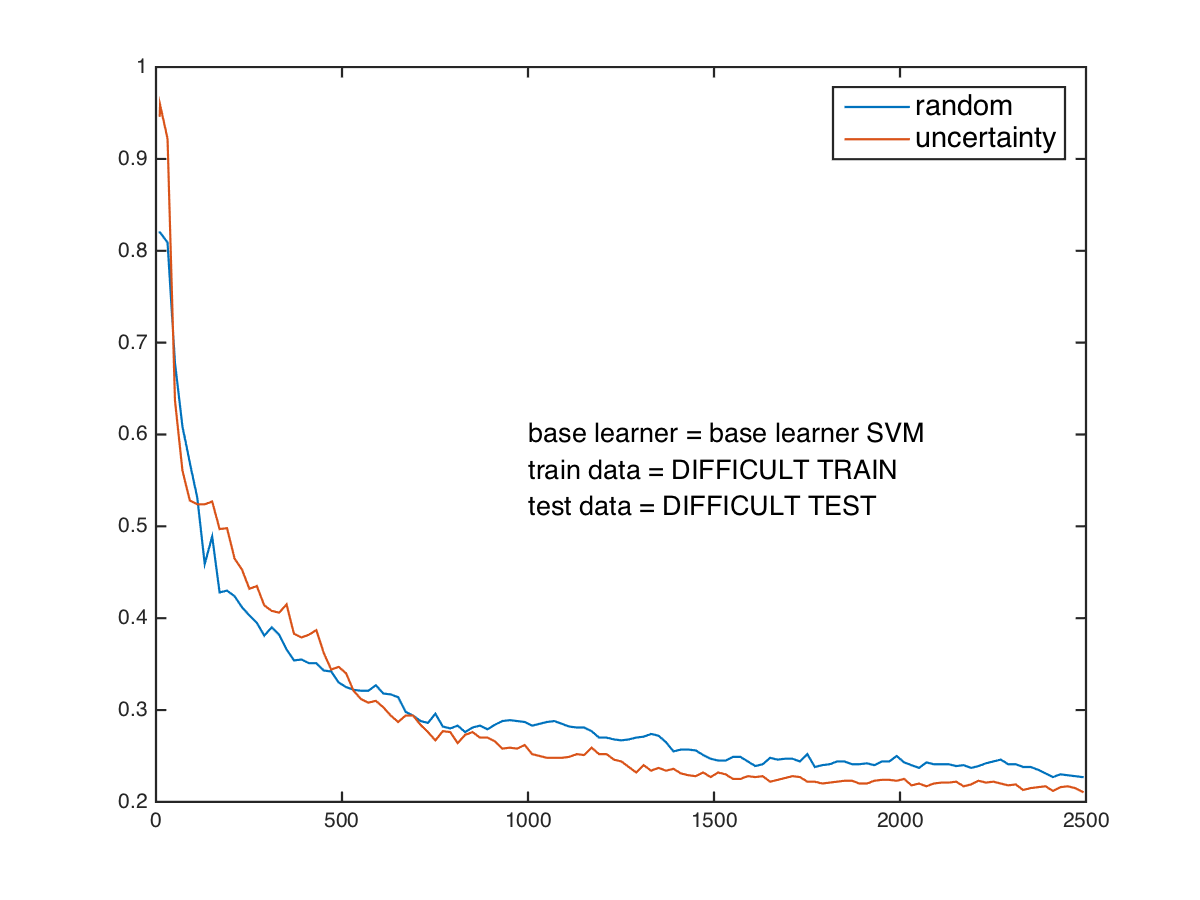
\includegraphics[width=1\linewidth]{../svm_difficult}
    \end{minipage}
    \caption{The results of SVM base learner (from left to right are the results of easy, moderate, and difficult datasets)}
    \label{fig:svm}
  \end{figure}

\subsection{Base learner - sparseLogit}

The results of uncertainty sampling with sparseLogit as base learner is shown in \Cref{fig:sparseLogit}. 
  \begin{figure}[!ht]
    \begin{minipage}{.31\textwidth}
      \centering
      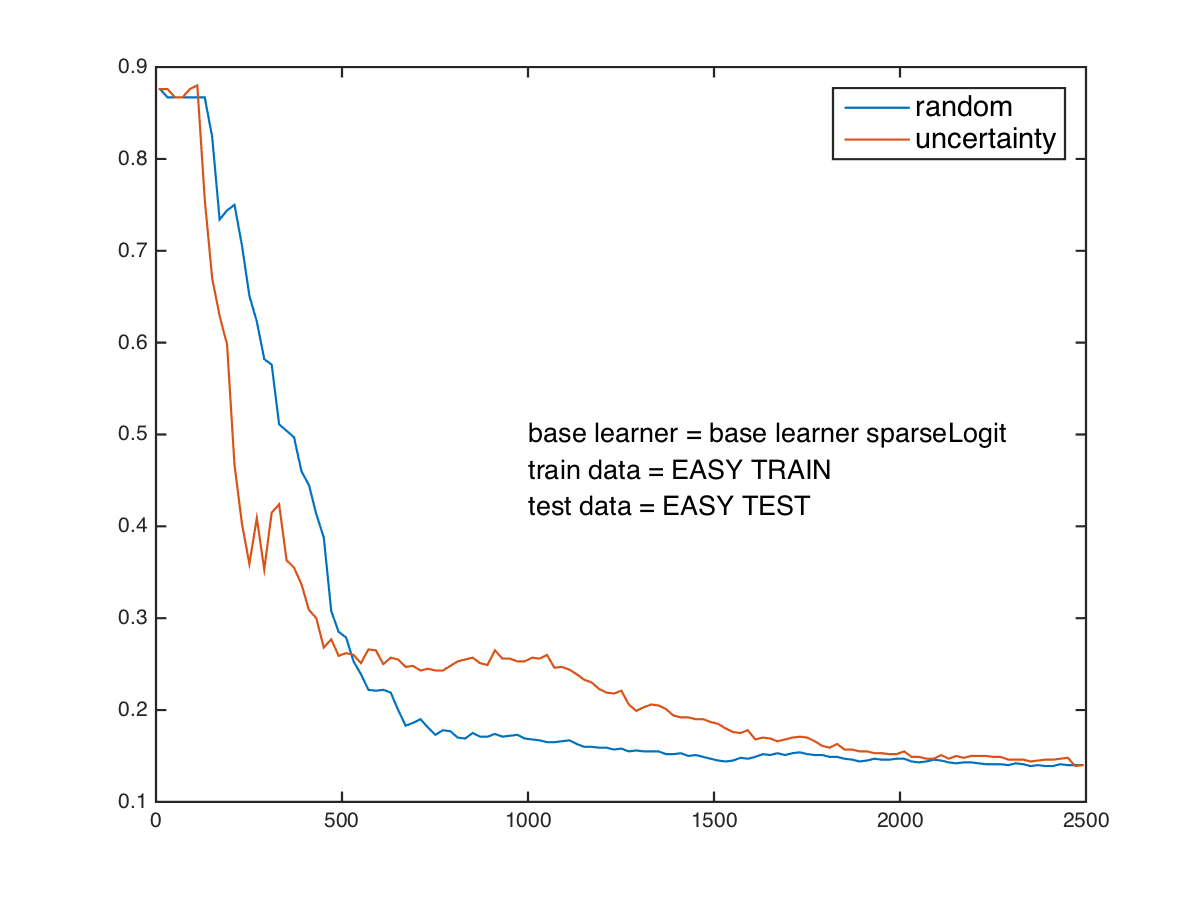
\includegraphics[width=1\linewidth]{../sparseLogit_simple}
    \end{minipage}
    \hfill
    \begin{minipage}{.31\textwidth}
      \centering
      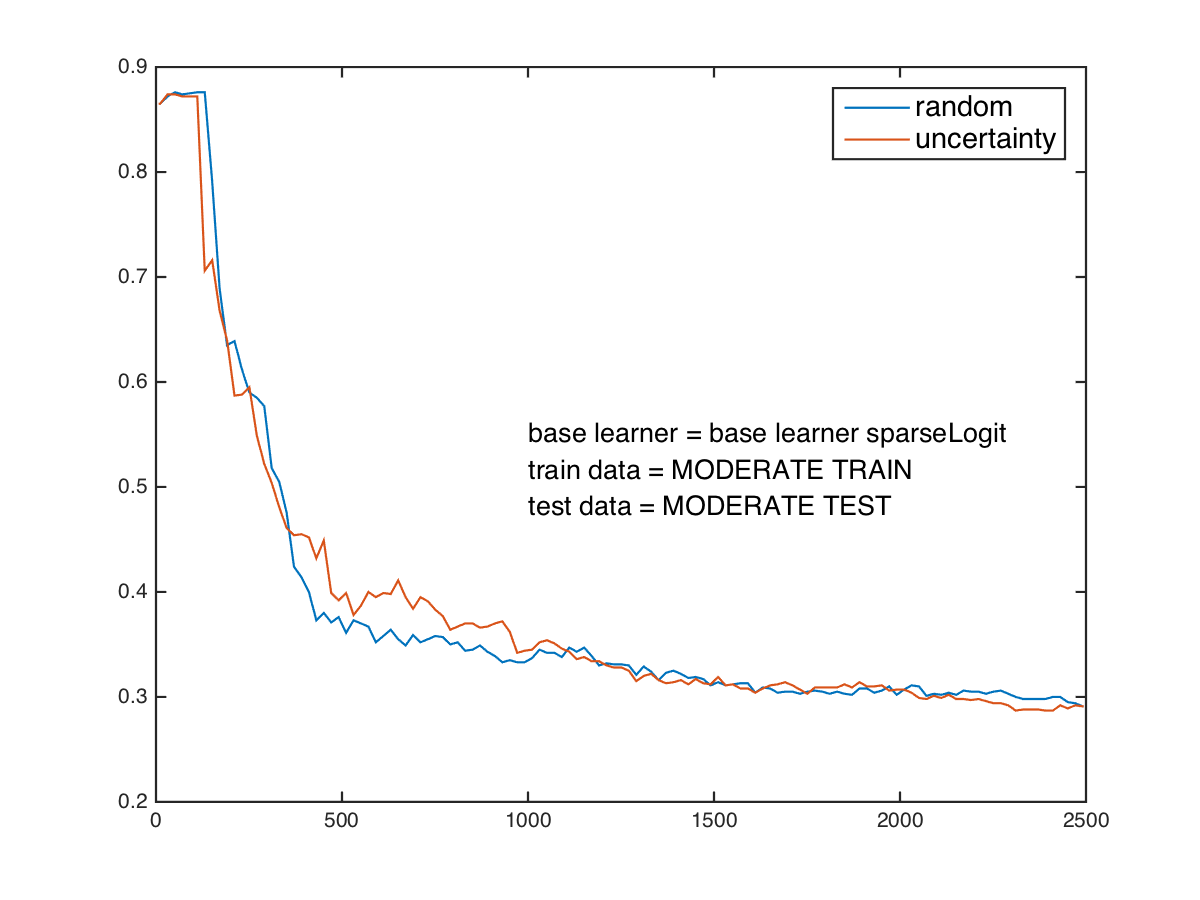
\includegraphics[width=1\linewidth]{../sparseLogit_moderate}
    \end{minipage}
    \hfill
    \centering
    \begin{minipage}{.31\textwidth}
      \centering
      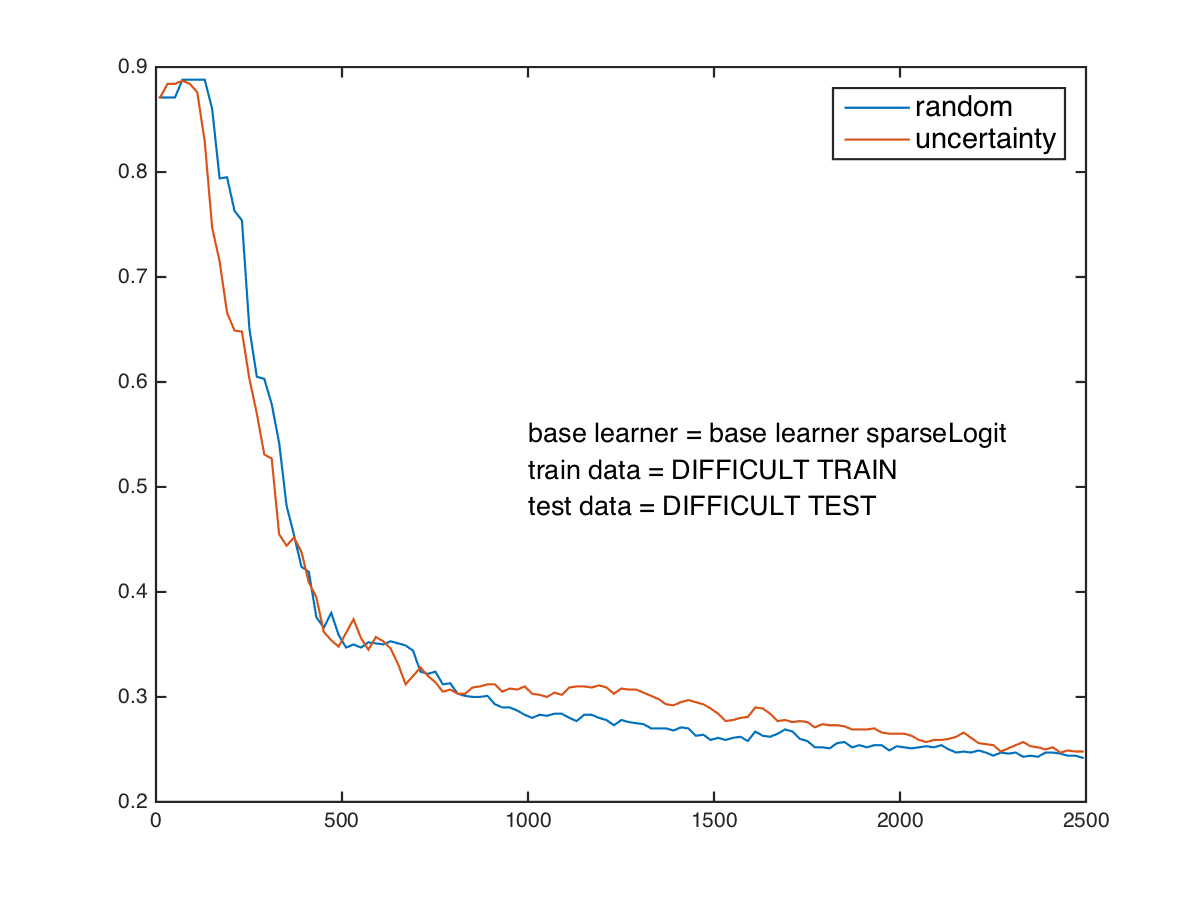
\includegraphics[width=1\linewidth]{../sparseLogit_difficult}
    \end{minipage}
    \caption{The results of sparseLogit base learner (from left to right are the results of easy, moderate, and difficult datasets)}
    \label{fig:sparseLogit}
  \end{figure}
The test error is high in sparseLogit, a possible reason of it is that the model complexity of sparseLogit is low (linear classifier), which might not be powerful enough for our datasets.

\subsection{Base learner - sparseNN}

The results of uncertainty sampling with sparseNN as base learner is shown in \Cref{fig:sparseNN}. 
  \begin{figure}[!ht]
    \begin{minipage}{.31\textwidth}
      \centering
      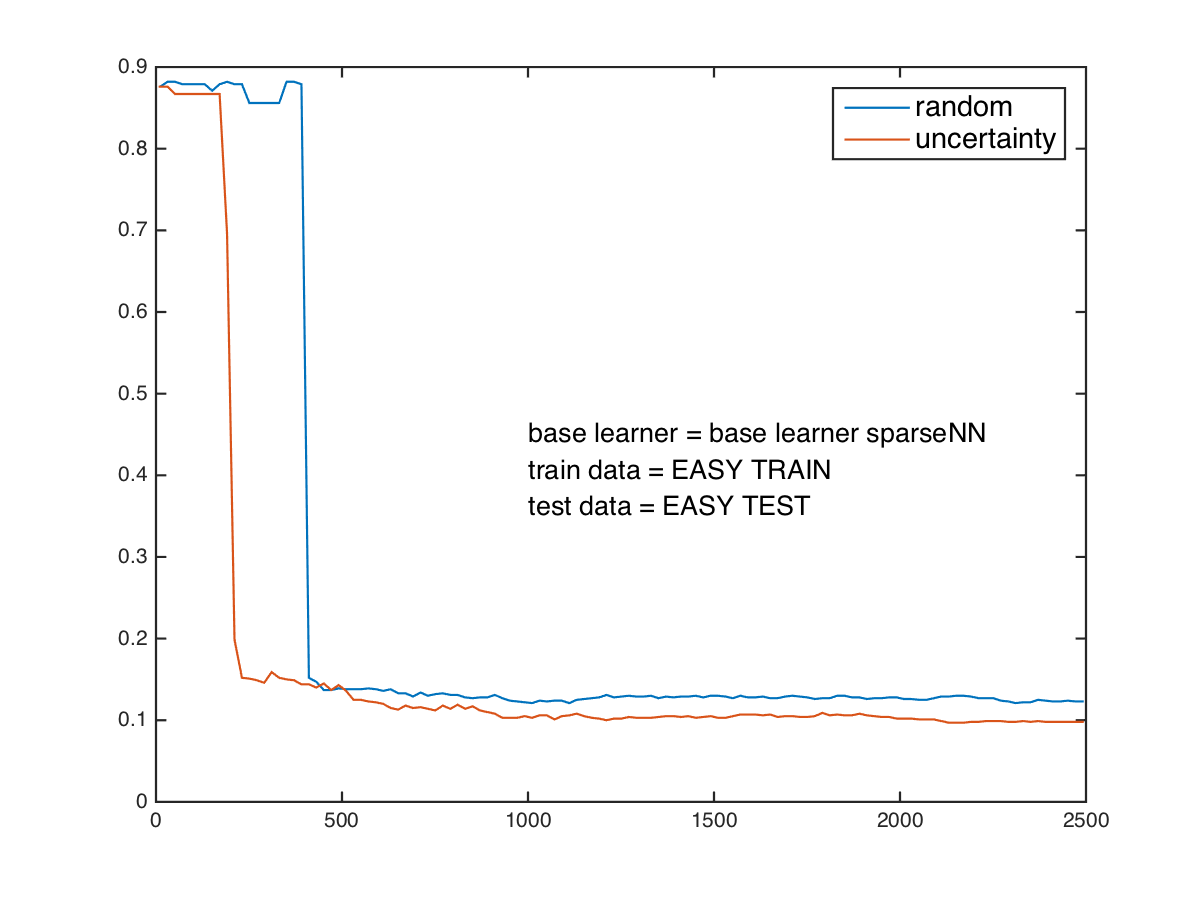
\includegraphics[width=1\linewidth]{../sparseNN_simple}
    \end{minipage}
    \hfill
    \begin{minipage}{.31\textwidth}
      \centering
      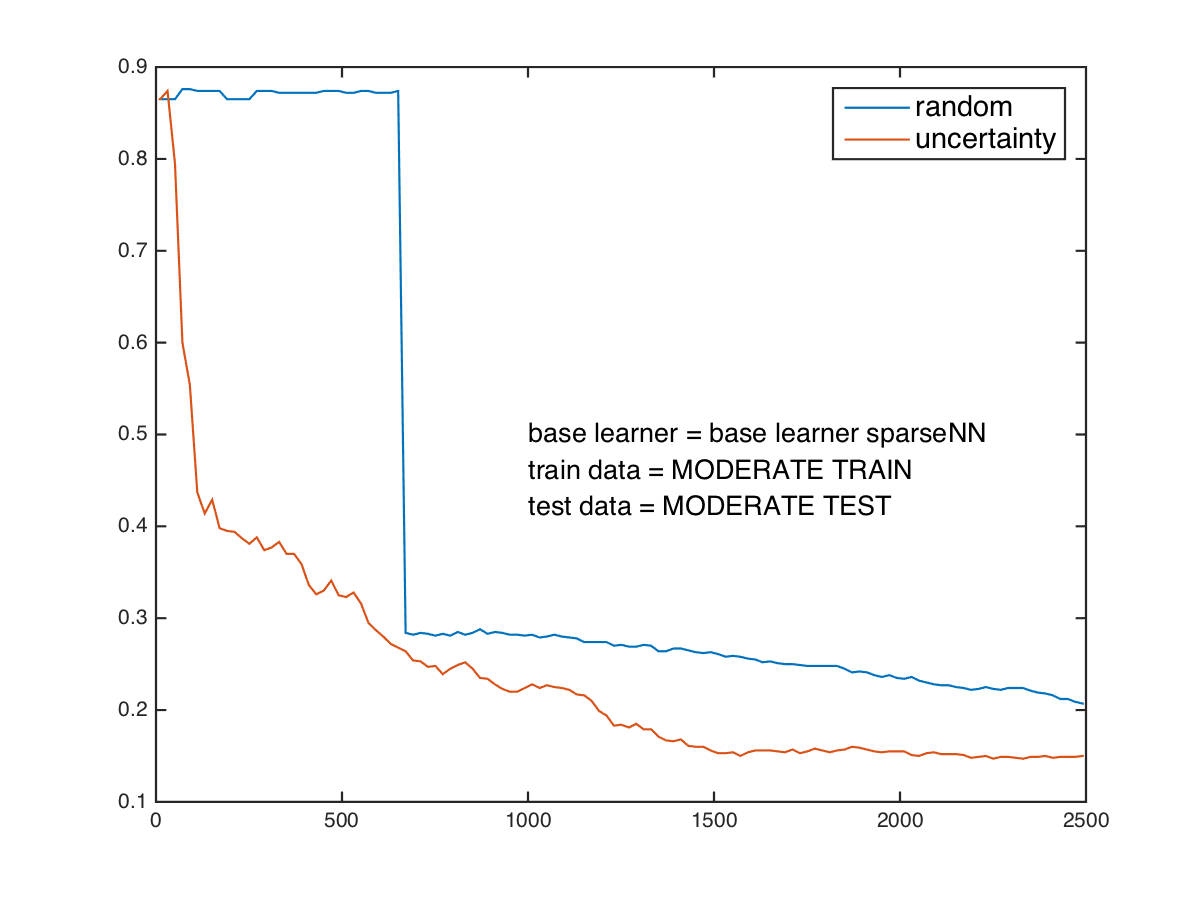
\includegraphics[width=1\linewidth]{../sparseNN_moderate}
    \end{minipage}
    \hfill
    \centering
    \begin{minipage}{.31\textwidth}
      \centering
      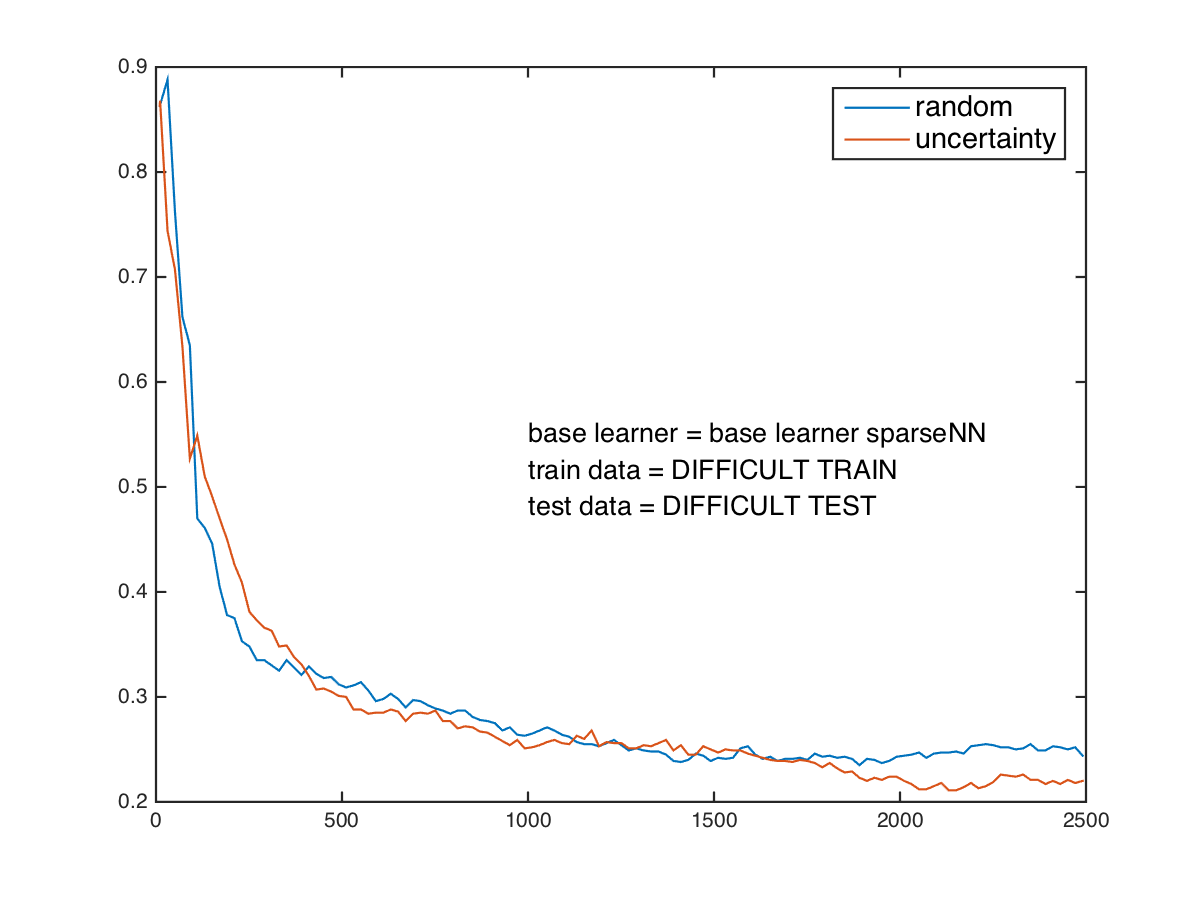
\includegraphics[width=1\linewidth]{../sparseNN_difficult}
    \end{minipage}
    \caption{The results of sparseNN base learner (from left to right are the results of easy, moderate, and difficult datasets)}
    \label{fig:sparseNN}
  \end{figure}
As an "advanced " or "deep" version of sparseLogit, sparseNN 

\section{Conclusion}

\bibliography{mybib}{}
\bibliographystyle{ieeetr}
\end{document}